%-----------------------------------------------------------------------
% Functional Programming 4
% John O'Donnell, Wim Vanderbauwhede
% University of Glasgow
%-----------------------------------------------------------------------

\documentclass{beamer}
\usepackage{jtodlecseriesFP4}

%include polycode.fmt
%format alpha = "\alpha"
%format ~> = "\leadsto "

% Identify this presentation
\SetPresentationTitle
  {Types}
  {Types}
\SetPresentationNumber
  {10}
\SetPresentationDate
  {Week 5-2}
  {Week 5-2}

%-----------------------------------------------------------------------
% Beginning

\begin{document}

\begin{frame}
  \PresentationTitleSlide
\end{frame}
%-----------------------------------------------------------------------
\begin{frame}
\begin{center}
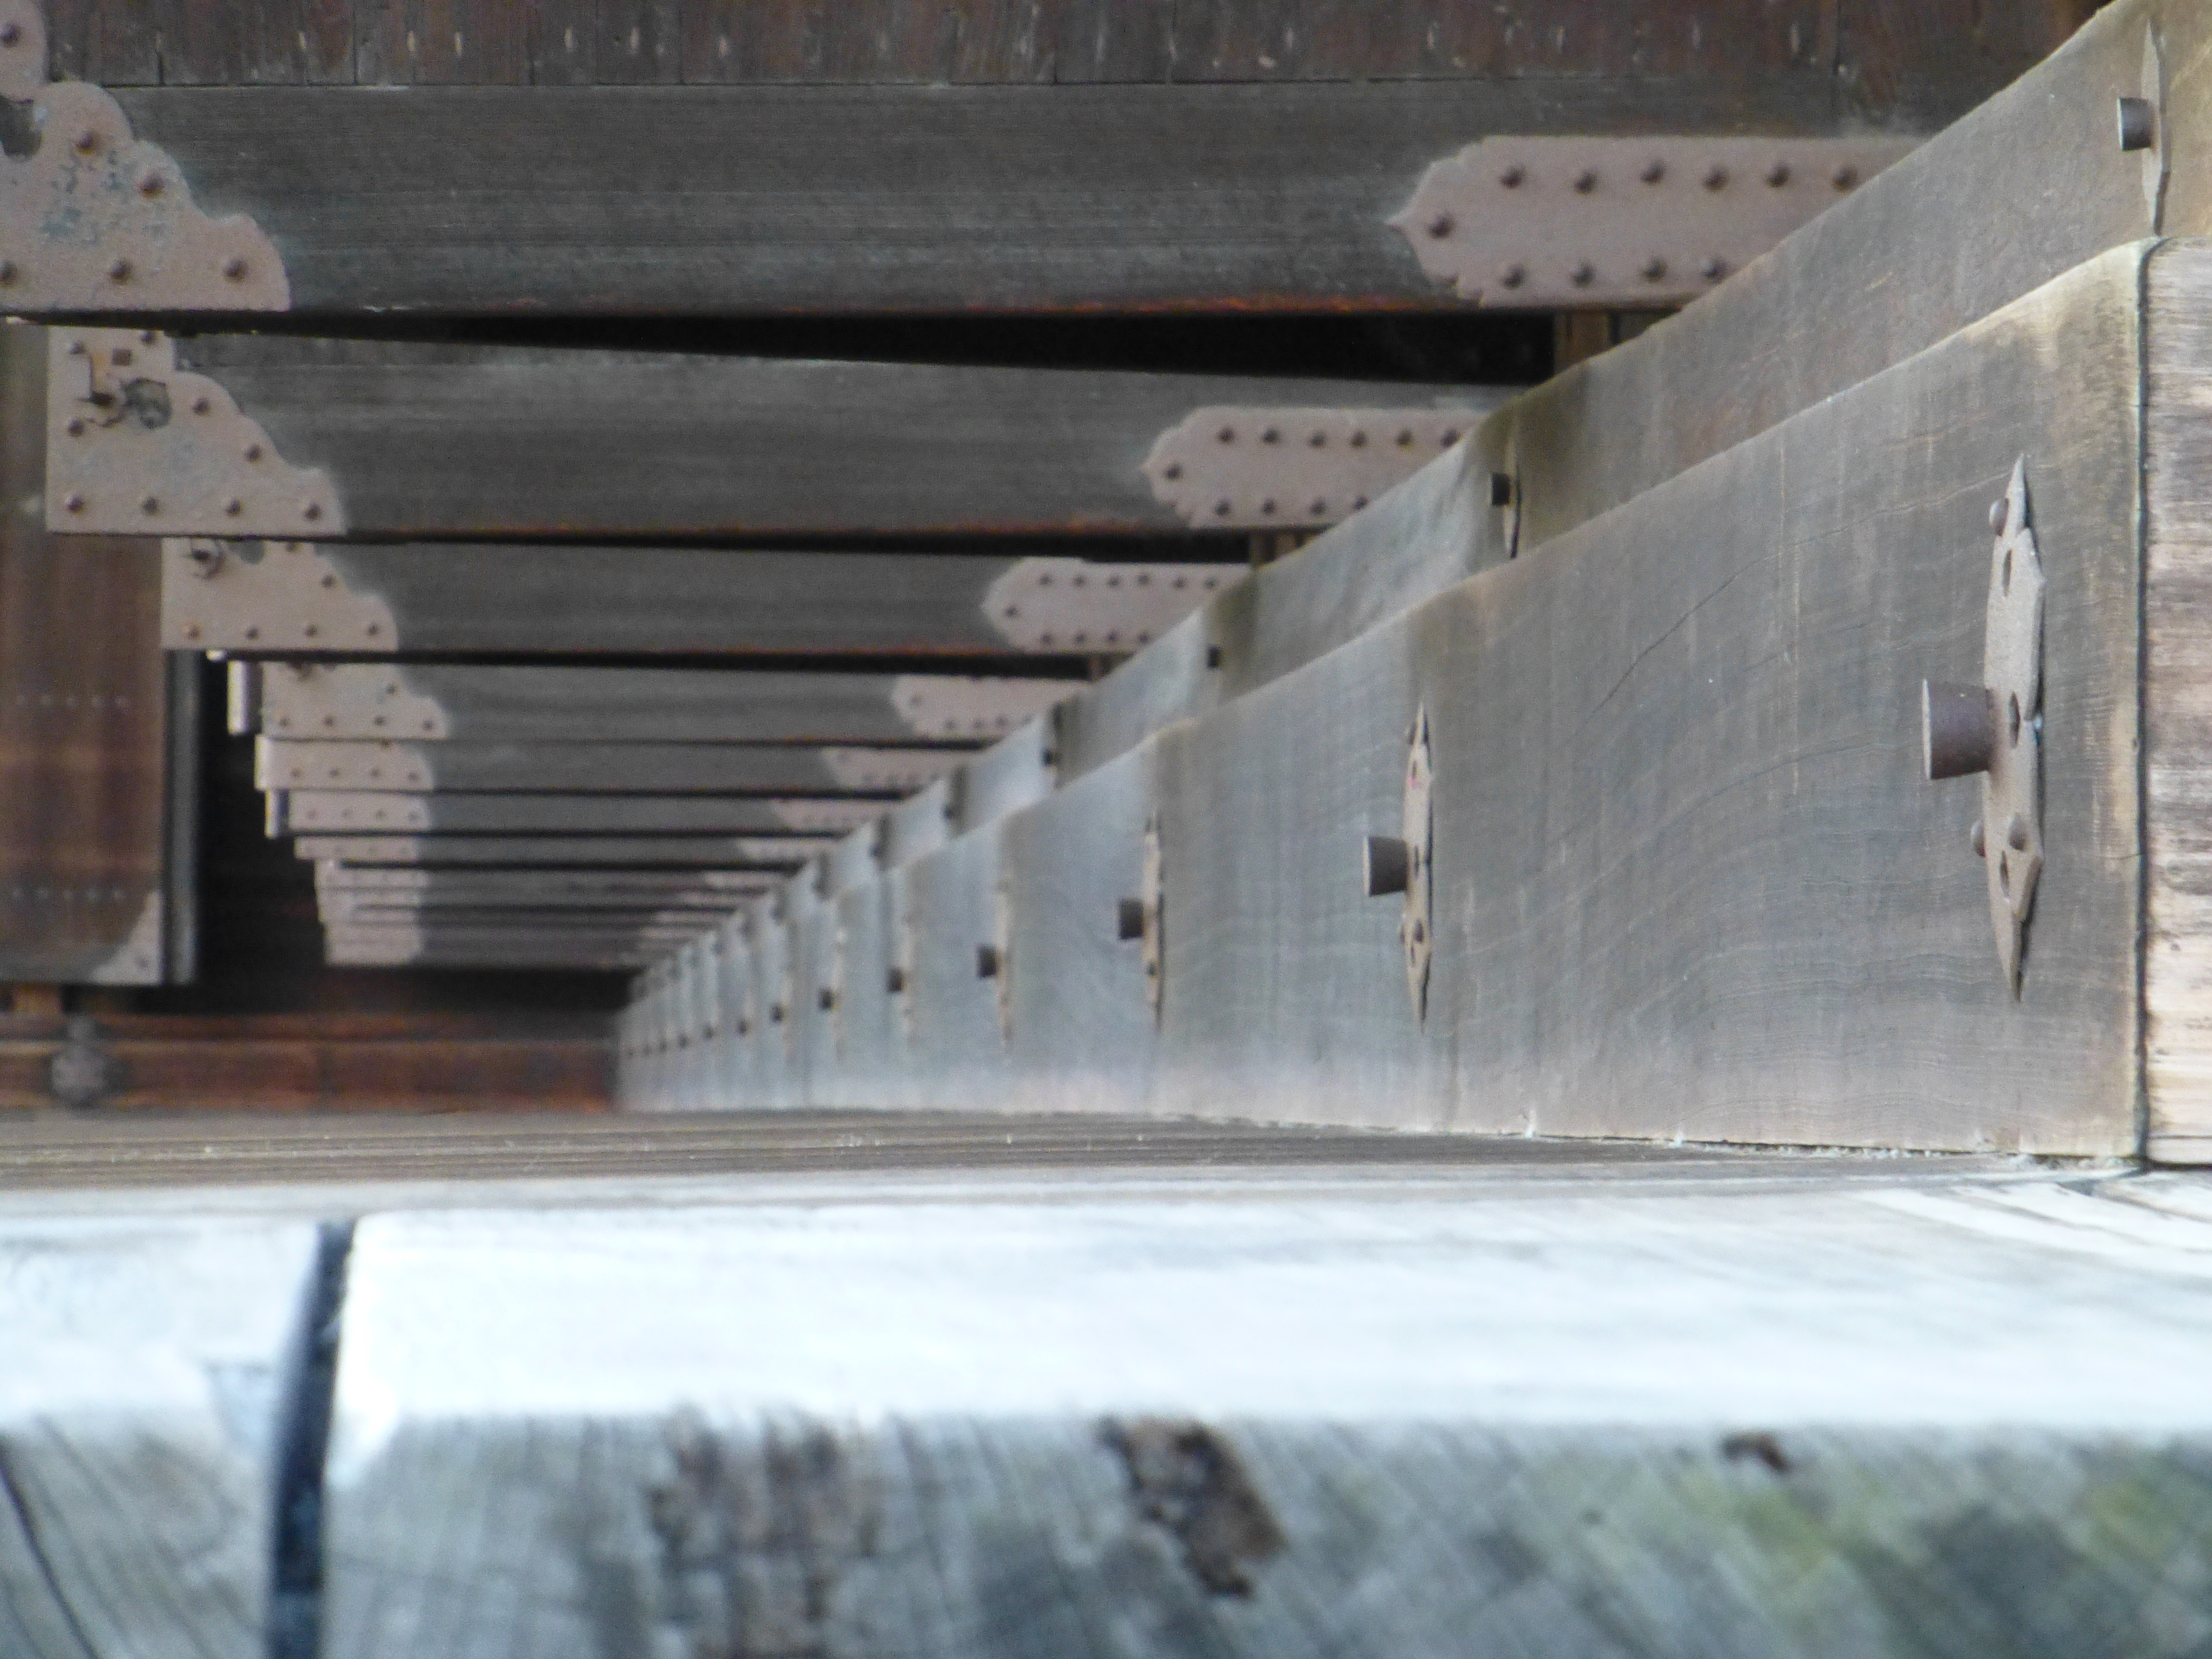
\includegraphics[scale=0.375]
    {figures/jpg/pic07.jpg}
\end{center}
\end{frame}

%-----------------------------------------------------------------------

\begin{frame}
  \frametitle{Topics}
  \tableofcontents
\end{frame}

%-----------------------------------------------------------------------
\section{Function types}

\begin{frame}
\frametitle{Function types}

\begin{itemize}
\item Ordinary data types are for primitive data (like $Int$ and
  $Char$) and basic data structures (like $[Int]$ and $[Char]$).
\item Functions have types containing an arrow, e.g. $Int \rightarrow
  String$.
\item We now look at function types in more detail.
\end{itemize}

\end{frame}

%-----------------------------------------------------------------------
\subsection{Lambda expressions}

\begin{frame}[fragile]
\frametitle{Named and anonymous expressions}

You can give a name $sum$ to an expression $2+2$:

\begin{verbatim}
sum = 2+2
\end{verbatim}

But you can also write \emph{anonymous expressions} --- expressions
that just appear, but are not given names.

\begin{verbatim}
(-b) + sqrt (b^2 - 4*a*c)
\end{verbatim}

Without anonymous expressions, writing this would almost be like
assembly language:

\begin{verbatim}
e1 = (-b)
e2 = b^2
e3 = 4*a
e4 = e3*c
e5 = e2-e4
e6 = e1+e5
\end{verbatim}

\end{frame}

%-----------------------------------------------------------------------
\begin{frame}
\frametitle{Some background}

\begin{itemize}
\item Sometimes in a mathematics or physics book, there are
  statements like ``the function $x^2$ is continuous$\ldots$''
\item This is ok when the context makes it clear what $x$ is.
\item But it can lead to problems.  What does $x*y$ mean?
  \begin{itemize}
  \item Is it a constant, because both $x$ and $y$ have fixed
    values?
  \item Is it a function of $x$, with a fixed value of $y$?
  \item Is it a function of $y$, with a fixed value of $x$?
  \item Is it a function of both $x$ and $y$?
  \end{itemize}
\item In mathematical logic (and computer programming) we need to
  be precise about this!
\item A lambda expression $\backslash x \rightarrow e$ contains
  \begin{itemize}
  \item An explicit statement that the formal parameter is $x$, and
  \item the expression $e$ that defines the value of the function.
  \end{itemize}
\end{itemize}

\end{frame}

%-----------------------------------------------------------------------
\begin{frame}[fragile]
\frametitle{Anonymous functions}

A function can be defined and given a name using an equation:

\begin{verbatim}
f :: Int -> Int
f x = x+1
\end{verbatim}

\begin{itemize}
\item Since functions are ``first class'', they are ubiquitous, and
  it's often useful to denote a function anonymously.
\item This is done using \emph{lambda expressions}.
\end{itemize}

\begin{verbatim}
\x -> x+1
\end{verbatim}

Pronounced ``lambda x arrow x+1''.

There may be any number of arguments:

\begin{verbatim}
\x y z -> 2*x + y*z
\end{verbatim}

\end{frame}

%-----------------------------------------------------------------------
\begin{frame}[fragile]
\frametitle{Using a lambda expression}

Functions are first class: you can use a lambda expression anywhere
a function is needed.  Thus

\begin{verbatim}
f = \x -> x+1
\end{verbatim}

is equivalent to

\begin{verbatim}
f x = x+1
\end{verbatim}

But lambda expressions are most useful when they appear inside
larger expressions.

\begin{verbatim}
map (\x -> 2*x + 1) xs
\end{verbatim}

\end{frame}

%-----------------------------------------------------------------------
\subsection{Monomorphic functions}

\begin{frame}[fragile]
\frametitle{Monomorphic functions}

Monomorphic means ``having one form''.

\begin{verbatim}
f :: Int -> Char
f i = "abcdefghijklmnopqrstuvwxyz" !! i
\end{verbatim}

\begin{verbatim}
x :: Int
x = 3
\end{verbatim}

\begin{verbatim}
f x :: Char
f x -- > 'c'
\end{verbatim}

\end{frame}

%-----------------------------------------------------------------------
\subsection{Polymorphic functions}
\begin{frame}[fragile]
\frametitle{Polymorphic functions}

Polymorphic means ``having many forms''.

\begin{verbatim}
fst :: (a,b) -> a
fst (x,y) = x
\end{verbatim}

\begin{verbatim}
snd :: (a,b) -> b
snd (x,y) = y
\end{verbatim}

\begin{verbatim}
fst :: (a,b) -> a
fst (a,b) = a
\end{verbatim}

\begin{verbatim}
snd :: (a,b) -> b
snd (a,b) = b
\end{verbatim}

\end{frame}

%-----------------------------------------------------------------------
\subsection{Currying}
\begin{frame}[fragile]
\frametitle{Currying}

\begin{itemize}
\item Most programming languages allow functions to have any number
  of arguments.
\item But this turns out to be unnecessary: we can restrict all
  functions to have just one argument, \emph{without losing any
    expressiveness}.
\item This process is called \emph{Currying}, in honor of Haskell
  Curry.
  \begin{itemize}
  \item The technique makes essential use of higher order
    functions.
  \item It has many advantages, both practical and theoretical.
  \end{itemize}
\end{itemize}

\end{frame}

%-----------------------------------------------------------------------
\begin{frame}[fragile]
\frametitle{A function with two arguments}

You can write a definition like this, which appears to have two
arguments:

\begin{verbatim}
f :: Int -> Int -> Int
f x y = 2*x + y
\end{verbatim}

But it actually means the following:

\begin{verbatim}
f :: Int -> (Int -> Int)
f 5 :: Int -> Int
\end{verbatim}

The function takes its arguments one at a time:

\begin{verbatim}
f 3 4 = (f 3) 4
\end{verbatim}

\begin{verbatim}
g :: Int -> Int
g = f 3
g 10 -- > (f 3) 10 -- > 2*3 + 10
\end{verbatim}

\end{frame}

%-----------------------------------------------------------------------
\begin{frame}[fragile]
\frametitle{Grouping: arrow to the right, application left}

\begin{itemize}
\item The arrow operator takes two types $a \rightarrow b$, and gives the type of a
  function with argument type $a$ and result type $b$
\item An application $e_1\; e_2$ applies a function $e_1$ to an
  argument $e_2$
\item Note that for both types and applications, \emph{a function
    has only one argument}
\item To make the notation work smoothly, arrows group to the
  right, and application groups to the left.
\end{itemize}

\begin{verbatim}
f :: a -> b -> c -> d
f :: a -> (b -> (c -> d))
\end{verbatim}

\begin{verbatim}
f x y z = ((f x) y) z
\end{verbatim}

\end{frame}

%-----------------------------------------------------------------------
\subsection{Type classes}
\begin{frame}[fragile]
\frametitle{The type of (+)}

Note that $fst$ has the following type, and there is no restriction
on what types $a$ and $b$ could be.

\begin{verbatim}
fst :: (a,b) -> a
\end{verbatim}

What is the type of $(+)$?  Could it be$\ldots$

\begin{verbatim}
(+) :: Int -> Int -> Int
(+) :: Integer -> Integer -> Integer
(+) :: Ratio Integer -> Ratio Integer -> Ratio Integer
(+) :: Double -> Double -> Double
\end{verbatim}

\begin{verbatim}
(+) :: a -> a -> a  -- Wrong! has to be a number
\end{verbatim}

\end{frame}

%-----------------------------------------------------------------------
\begin{frame}[fragile]
\frametitle{Type classes}

Answer: $(+)$ has type $a \rightarrow a \rightarrow a$ for any type $a$ that is a
member of the type class $Num$.

\begin{verbatim}
(+) :: Num a => a -> a -> a
\end{verbatim}

\begin{itemize}
\item The class $Num$ is a set of types for which $(+)$ is defined
\item It includes $Int$, $Integer$, $Double$, and many more.
\item But $Num$ does \emph{not} contain types like $Bool$,
  $[Char]$, $Int->Double$, and many more.
\end{itemize}

\end{frame}

%-----------------------------------------------------------------------
\begin{frame}[fragile]
\frametitle{Two kinds of polymorphism}

\begin{itemize}
\item \emph{Parametric polymorphism.}
  \begin{itemize}
  \item A polymorphic type that can be instantiated to \emph{any}
    type.
  \item Represented by a type variable.  It is conventional to use
    $a$, $b$, $c$, $\ldots$
  \item Example: $length :: [a] \rightarrow Int$ can take the length of a
    list whose elements could have any type.
  \end{itemize}

\item \emph{Ad hoc polymorphism.}
  \begin{itemize}
  \item A polymorphic type that can be instantiated to any type
    chosen from a set, called a ``\emph{type class}''
  \item Represented by a type variable that is constrained using
    the $\Rightarrow$ notation.
  \item Example: $(+) :: Num a \Rightarrow a \rightarrow a \rightarrow a$ says that $(+)$ can
    add values of any type $a$, provided that $a$ is an element of
    the type class $Num$.
  \end{itemize}
\end{itemize}

\end{frame}

%-----------------------------------------------------------------------
\section{Type inference}
\begin{frame}[fragile]
\frametitle{Type inference}

\begin{itemize}
\item \emph{Type checking} takes a type declaration and some code,
  and determines whether the code actually has the type declared.
\item \emph{Type inference} is the analysis of code in order to
  infer its type.
\item Type inference works by
  \begin{itemize}
  \item Using a set of \emph{type inference rules} that generate
    typings based on the program text
  \item Combining all the information obtained from the rules to
    produce the types.
  \end{itemize}
\end{itemize}

\end{frame}

%-----------------------------------------------------------------------
\begin{frame}[fragile]
\frametitle{Type inference rules}

The type system contains a number of \emph{type inference rules},
with the form

\infrule[]
  {\hbox{assumption --- what you're given}}
  {\hbox{consequence --- what you can infer}}

\end{frame}

%-----------------------------------------------------------------------
\begin{frame}[fragile]
\frametitle{Context}

\begin{itemize}
\item Statements about types are written in the form similar to
  $\Gamma \vdash e :: \alpha$
\item This means ``if you are given a set $\Gamma$ of types, then
  it is proven that $e$ has type $\alpha$.
\end{itemize}

\end{frame}

%-----------------------------------------------------------------------
\begin{frame}[fragile]
\frametitle{Type of constant}

\infrule[]
  {\hbox{$c$ is a constant with a fixed type $T$}}
  {\Gamma \vdash c :: T}

\vspace{2em}

If we know the type $T$ of a constant $c$ (for example, we know that $'a'
:: Char$), then this is expressed by saying that there is a given
theorem that $c :: T$.  Furthermore, this holds given \emph{any}
context $\Gamma$.

\end{frame}

%-----------------------------------------------------------------------
\begin{frame}[fragile]
\frametitle{Type of application}

\infrule[]
  {\Gamma \vdash e_1 :: (\alpha \rightarrow \beta)
   \qquad
   \Gamma \vdash e_2 :: \alpha
  }
  {\Gamma \vdash (e_1 \ e_2) :: \beta}

\vspace{2em}

If $e_1$ is a function with type $\alpha \rightarrow \beta$, then
the application of $e_1$ to an argument of type $\alpha$ gives a
result of type $\beta$.

\end{frame}

%-----------------------------------------------------------------------
\begin{frame}[fragile]
\frametitle{Type of lambda expression}

\infrule[]
  {\Gamma, x :: \alpha \quad \vdash \quad e :: \beta}
  {\Gamma \vdash (\lambda x \rightarrow e)
     :: (\alpha \rightarrow \beta)}

\vspace{2em}

We have a context $\Gamma$.  Suppose that if we're also given that
$x :: \alpha$, then it can be proven that an expression $e ::
\beta$.  Then we can infer that the function $\lambda x \rightarrow
e$ has type $\alpha \rightarrow \beta$.

\end{frame}

\end{document}
